\section{Tábua de Logaritmo}


A capacidade computacional hodierna banalizou operações que antes representavam desafios consideráveis de tempo e precisão, como o produto $4538 \cdot 675$. Entretanto, até a disseminação das calculadoras eletrônicas na década de 1970, tal cálculo exigia métodos analógicos e tabulares. Na época, a solução era advinda de métodos que utilizavam tábuas de logaritmos e réguas de cálculo.

\begin{figure}[H]
    \centering
    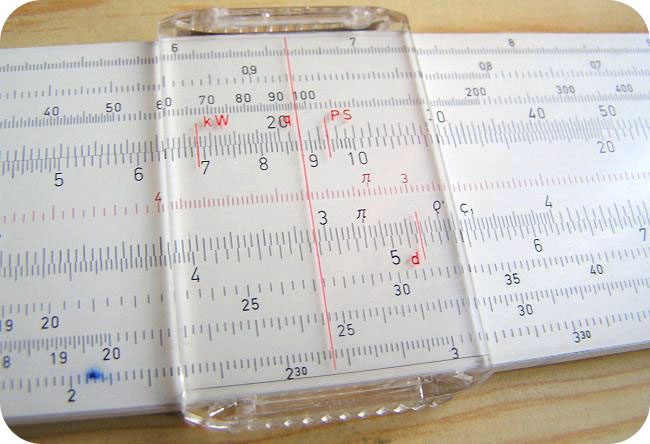
\includegraphics[height=6cm]{img/regua.png}
    \caption{Régua de Cálculo}
\end{figure}

\subsection{Exemplo}

Para elucidar o método, demonstraremos como as tábuas eram utilizadas para computar o produto $4538\cdot 675$. O método se fundamenta a partir da seguinte propriedade de logaritmo:

\begin{align*}
    P = a \cdot b \quad & \implies \quad \log(P) = \log(a \cdot b) \\
                       & \implies \quad \log(P) = \log(a) + \log(b) \\
                       & \implies \quad P = \log^{-1}\left( \log(a) + \log(b) \right)
\end{align*}

\textbf{Tabelas do Exemplo:}
\begin{figure}[H]
    \centering
    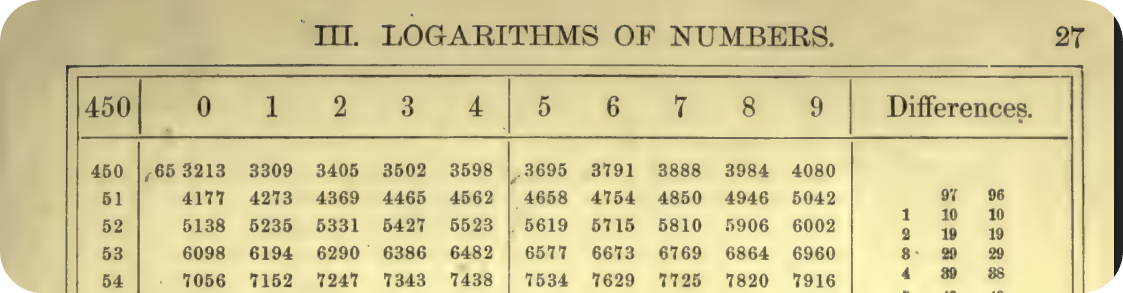
\includegraphics[height=3cm]{img/4538.png}
    \caption{Tabela do Número 4538}
\end{figure}

\begin{figure}[H]
    \centering
    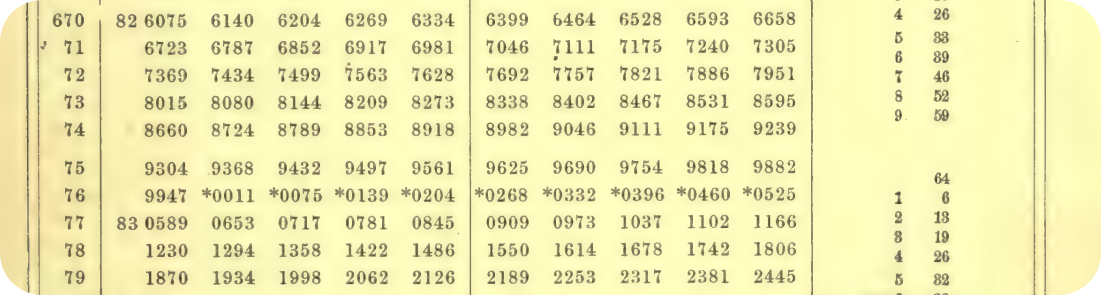
\includegraphics[height=3cm]{img/675.png}
    \caption{Tabela do Número 675}
\end{figure}

\begin{figure}[H]
    \centering
    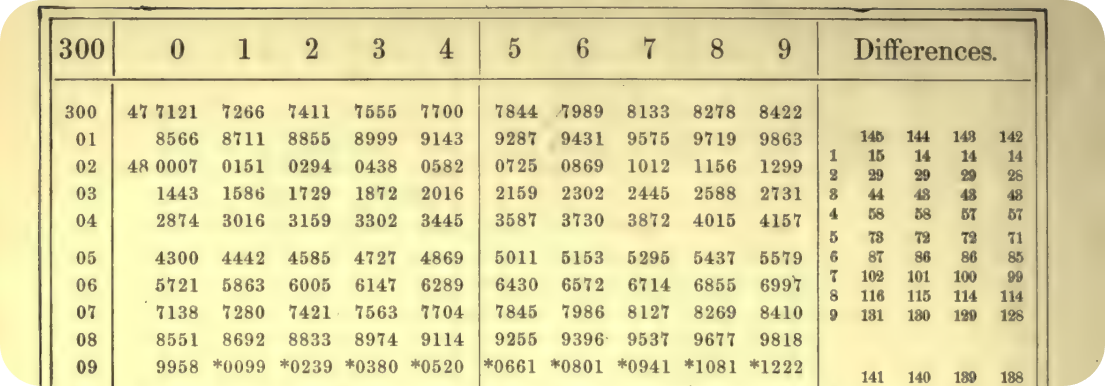
\includegraphics[height=4cm]{img/res.png}
    \caption{Tabela do Número Resultado}
\end{figure}

Para fins de organização separemos o método em etapas:

\begin{itemize}
    \item Passo 1: Computar o logaritmo dos números 4538 e 675
    \item Passo 2: Somar o resultado encontrado
    \item Passo 3: Encontrar o antilogaritmo do resultado
    \item Passo 4: Aplicar métodos de interpolação para melhorar o resultado.
\end{itemize}

\subsubsection{Passo 1}
A princípio, é necessário computar o logaritmo dos número 4538 e 675. Mostraremos o processo para o número 4538 e para o número 675 é análogo e fica como exercício para o leitor. O método pode ser particionado em encontrar a parte inteira e a parte fracionária do logaritmo desejado, denota-se característica e mantissa respectivamente.

\textbf{Parte Inteira:}
Note que:
\begin{align*}
    & 10^3 \le 4538 \le 10^4 \iff \\
    & \log(10^3) \le \log(4538) \le \log(10^4) \iff \\
    & 3 \le \log(4538) \le 4
\end{align*}

Daí, a parte inteira do $\log(4538)$ é 3.

\textbf{Mantissa:}
Para a mantissa é necessário consultar a tábua presente na Figura 2. Em suma, basta encontrar os primeiros digitos do valor desejado (450) e veja que os algarismos da parte superior da tábua é referente ao último digito, isto é, no exemplo devemos consultar a coluna do 8. Além disso, nesse exemplar é omitido as duas primeiras casas decimais da mantissa, nessa tábua tais valores estão precedentes à coluna do algarismo 0, isto é, no exemplo, já juntando os digitos, a mantissa é 656864.

Para descobrir a mantissa do valor 675 faça o uso da tábua presente na Figura 3.

Daí, $\log(4538) \approx 3,656864$ e $\log(675) \approx 2,829304$.

\subsubsection{Passo 2}

Somando os valores encontrados no passo anterior, temos que:
\begin{align*}
    \log(4538 \cdot 675) &= \log(4538) + \log(675) \\
                        &\approx 3{,}656864 + 2{,}829304 \\
                        &= 6{,}486168
\end{align*}

\subsubsection{Passo 3}
De maneira análoga, encontrar o antilogaritmo segue o mesmo método.

\textbf{Parte Inteira:}

\begin{align*}
    & 6 \le 6{,}486168 \le 7 \iff \\
    & \log^{-1}(6) \le \log^{-1}(6{,}486168) \le \log^{-1}(7) \iff \\
    & 10^6 \le 4538 \cdot 675 \le 10^7
\end{align*}

Daí, a parte inteira indica que o resultado está na casa dos milhões ($10^6$).

\textbf{Mantissa:}
Por meio da tábua na Figura 4, procuremos os dois primeiros digitos da mantissa (48), como logaritmo é uma função crescente, basta procurar ordenadamente. Daí, nos valores que englobam o 48 procuremos pelo piso de 6168. Veja que, como não há o número exato, o número se encontra no intervalo $[6147, 6289]$. Assim, ao tomar 6147 encontramos que o valor aproximado do antilogaritmo desejado é 3063.

Juntando a informação obtida a partir da parte inteira e da mantissa chegamos que $4538 \cdot 675 = 3.063.000$. Por meio de ferramentas de computacionais hodierna descobrimos que o produto é na verdade 3063150; assim, o erro percentual relativo é 0,0049\% .

\subsubsection{Passo 4}

Não satisfeito com a aproximação anterior, ainda por meio da tábua há a possibilidade de melhorar o resultado.

No passo precedente, vimos que $6168 \in I=[6147, 6289]$, assim, $|I| = 142$ e a diferença do valor desejado para o extremo esquerdo de I é $6168-6147 = 21$. Dessa maneira, analisando a parte de diferença da tabela na coluna $142$, vemos que $21 \in [14,28]$, melhor dizendo, o quinto dígito é 1, já que devemos sempre pegar o mínimo do menor intervalo possível. Assim, o resultado do produto se torna 3.063.100.

Para descobrirmos o sexto dígitos é necessário realizar um truque, note que no processo anterior na tabela das diferenças não encontramos exatamente o número 21, então podemos subtrair o valor desejado pelo extremo esquerdo do intervalo, $21-14 = 7$ (denotaremos de resto). Além disso, computamos o tamanho do intervalo, isto é, $28-14 = 14$ (denotaremos de intervalo). Daí, utilizando a seguinte fórmula:

\begin{align*}
    \dfrac{Resto}{Intervalo} = 7/14 = 0.5
\end{align*}

O resultado nos dá o sexto digito, assim, o resultado do produto se torna 3.063.150

\subsubsection{Conclusão}
Veja que após realizar o processo de interpolação duas vezes consecutivas reduzimos o erro percentual relativo para zero, isto é, encontramos o resultado exato. Demonstrando que apesar de trabalhoso o método realmente é funcional.